\subsubsection{Validación del modelo de predicción}

A continuacion, se presentan los resultados obtenidos en la validación del modelo de predicción. Estos resultados se obtuvieron luego de aplicar la estrategia de validacion ya definida anteriormente, sobre el historial real de consumo de 856 productos (medicamentos) del año 2021 - 2022 en la Clinica Nuestra Señora de los remedios. 

Las metricas obtenidas al evaluar los tres modelos candidatos, junto con el metodo de seleccion de modelo por producto. Todo esto sobre el ultimo periodo de prueba disponible, que corresponde a junio 2022, con seis meses de entrenamiento previo.

\begin{table}[H]
    \centering
    \caption{Métricas del holdout final por modelo.}
    \label{tab:resultados_holdout}
    \begin{tabularx}{\textwidth}{Xcccc}
        \toprule
        \textbf{Modelo} & \textbf{MAE} & \textbf{RMSE} & \textbf{MAPE (\%)} & \textbf{WAPE (\%)} \\
        \midrule
        Media Móvil (3 meses) & 48.79 & 243.65 & 80.32 & 23.86 \\
        Regresión Lineal      & 56.43 & 276.41 & 95.30 & 27.60 \\
        XGBoost (log1p)       & 50.59 & 254.82 & 65.12 & 24.74 \\
        \textbf{Sistema final (selección por producto)} & \textbf{39.60} & \textbf{207.14} & \textbf{57.63} & \textbf{19.37} \\
        \bottomrule
    \end{tabularx}
\end{table}

\begin{figure}[H]
    \centering
    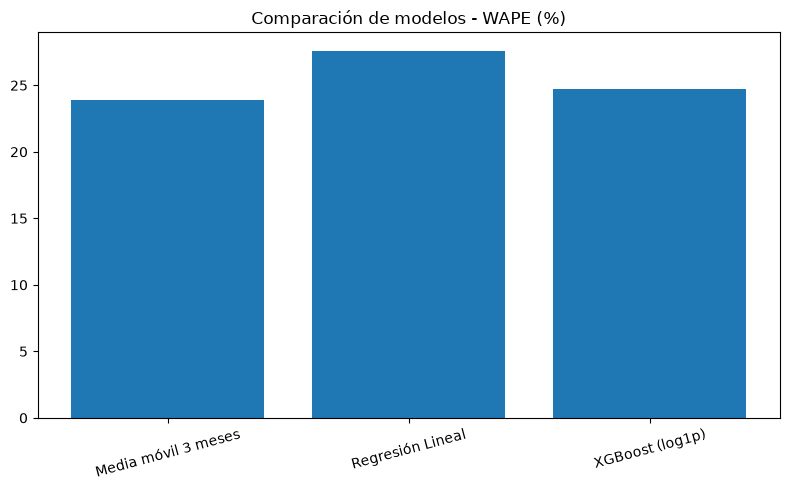
\includegraphics[width=0.75\textwidth]{templatefigures/comparacion_WAPE_porcentaje}
    \caption{Comparación de WAPE entre los tres modelos candidatos (holdout final).}
    \label{fig:comparacion_wape}
\end{figure}

\subsubsection{Consistencia mediante validación cruzada temporal}

Despues de obtener los resultados anteriores, se propuso el uso de una validacion cruzada para descartar que el resultado obtenido dependiera de las condiciones y particularidades de un unico periodo de prueba.

La idea principal, es probar el modelo varias veces simulando estar en un mes distinto al pasado, para poder evaluar si acierta de forma consistente y no solo una vez por casualidad. Para poder predecir un mes, solo se puede usar los meses que vinieron antes, no se pueden usar los datos que serian "Futuros", porque queremos simular un escenario real, y en ese caso, no se tendria esa informacion.


\begin{enumerate}
    \item Prueba 1 (Fold 1): Es el mas antiguo, se le enseña al modelo con los primeros 4 meses del año (Enero, febrero, Marzo, Abril), y se hace que el sistema adivine Mayo, Junio y Julio. Se compara lo que adivino contra los resultados reales de esos meses y se registra que tan grande fue el error.
    \item Prueba 2 (Fold 2): En este segunda prueba o Fold, se le enseña al modelo con 5 meses en ves de 4, es decir, de enero a Mayo, y se le pide que prediga Junio, Julio y agosto, una vez mas, se comparar y se registra el error.
    \item Prueba 3 (Fold 3): Por ultimo, se le enseña al modelo con 6 meses de Enero a junio y se le solicita al sistema que prediga julio , agosto y septiembre, se compara y, una vez mas, se registra el error.
\end{enumerate}


Dicha validacion cruzada temporal se implemento en el sistema en el archivo \texttt{app/services/prediccion/validacion.py}.

\begin{minted}{python}
TEST_SIZE_MESES = 3
MIN_TRAIN_MESES = 3
MAX_FOLDS = 3


def _armar_folds(meses_ordenados):
    n = len(meses_ordenados)
    folds = []
    fin_test = n
    while len(folds) < MAX_FOLDS:
        inicio_test = fin_test - TEST_SIZE_MESES
        if inicio_test < MIN_TRAIN_MESES:
            break
        folds.append((meses_ordenados[:inicio_test], meses_ordenados[inicio_test:fin_test]))
        fin_test -= 1
    folds.reverse()
    return folds
\end{minted}

Se definen tres constantes, \texttt{TEST\_SIZE\_MESES}, \texttt{MIN\_TRAIN\_MESES} y \texttt{MAX\_FOLDS}, que definen el tamaño de la ventana de prueba, el tamaño minimo de la ventana de entrenamiento y el numero maximo de folds a generar, respectivamente.


Se arma la funcion que genera las particiones \texttt{\_armar\_folds}, esta recibe una lista de todos los meses disponibles organizados cronologicamente. Se define el fold mas reciente, es decir, los ultimos meses disponibles \texttt{TEST\_SIZE\_MESES}. En cada iteracion se retrocede el punto de corte de un mes hacia atras en el tiempo, de esta manera, se crea un nuevo Fold cuyo entrenamiento crece en un mes respecto al anterior. Este proceso se repite hasta completar \texttt{MAX\_FOLDS}, o hasta que ya no quede suficiente historial y el tamaño de la ventana de entrenamiento sea menor a \texttt{MIN\_TRAIN\_MESES} meses de entrenamiento.  

Al finalizar, los folds se ordenan en orden cronologico del mas antiguo al mas nuevo antes de ser devueltos.

Al ya tener los folds organizados, el sistema entrena nuevamente los tres modelos candidatos, y selecciona el mejor modelo por producto, evaluando el resultado bajo la etiqueta de "Sistema final". Es decir, es la estrategia que usa Thary para predecir el consumo, en ves de escoger uno solo, para cada producto, el sistema entrena los 3 modelos y selecciona el que se equivoco menos conese producto en particular. El proceso se repite producto por producto.

Un aspecto importante es que, la eleccion de que modelo usar para cada producto se hace solo con los datos de entrenamiento, antes de ver los datos de prueba. Esto demuestra que no se esta "haciendo trampa, ya que el sistema no tiene acceso a los datos de prueba, y por lo tanto, no puede "aprender" de ellos.

Aun asi, solo esto no basta para confiar en el resultado, ya que aun si el sistema esta eligiendo el modelo de forma honesto, un unico experimento podria haber salido bien por casualidad y no porque el sitema de verdad sea bueno.


Es por eso que la validacion cruzada la aporto valor al sistema, ya que al repetir este mismo proceso (entrenamiento, eleccion del modelo y evaluacion) en diferentes periodos de prueba, se confirma que el resultado obtenido en el holdout final no fue un resultado aislado, sino que se repite de forma consistente en distintos periodos de prueba.

En la siguiente tabla se describen el promedio y la desviiacion estandar de las metricas obtenidas en cada fold, para cada modelo candidato y el sistema final:


\begin{table}[H]
    \centering
    \caption{Resumen de la validación cruzada temporal (promedio $\pm$ desviación, 3 folds).}
    \label{tab:resumen_cv}
    \begin{tabularx}{\textwidth}{Xcccc}
        \toprule
        \textbf{Modelo} & \textbf{MAE} & \textbf{RMSE} & \textbf{MAPE (\%)} & \textbf{WAPE (\%)} \\
        \midrule
        Media Móvil        & 44.27 $\pm$ 3.70  & 200.82 $\pm$ 41.31 & 82.38 $\pm$ 1.85  & 22.31 $\pm$ 1.29 \\
        Regresión Lineal   & 58.13 $\pm$ 2.21  & 270.35 $\pm$ 6.32  & 106.24 $\pm$ 10.64 & 29.38 $\pm$ 1.84 \\
        XGBoost            & 46.58 $\pm$ 3.46  & 223.64 $\pm$ 31.40 & 64.93 $\pm$ 2.25  & 23.48 $\pm$ 1.15 \\
        \textbf{Sistema final} & \textbf{36.25 $\pm$ 2.54} & \textbf{174.24 $\pm$ 27.89} & \textbf{59.13 $\pm$ 1.84} & \textbf{18.27 $\pm$ 0.81} \\
        \bottomrule
    \end{tabularx}
\end{table}

De la tabla se puede observar que:

De la tabla se puede observar que:

\begin{itemize}
    \item El sistema final es el que obtiene el mejor promedio en las cuatro metricas evaluadas, y tambien la menor desviacion estandar en todas ellas. Esto es significativo, porque demuestra que vale la pena la complejidad de elegir un modelo distinto para cada producto: el sistema final no solo es mas preciso en promedio, sino tambien mas consistente y estable entre los distintos periodos evaluados.
    \item La media movil es el segundo mejor modelo, seguido por XGBoost y finalmente la regresion lineal. Cuando se comparan los tres modelos candidatos de forma individual, la media movil es la que obtiene un mejor MAE, RMSE y WAPE, mientras que solo XGBoost la supera en MAPE. El hecho de que ninguno de los dos modelos mas sofisticados domine de forma general sobre la linea base avala la decision de seleccionar un modelo distinto por producto, ya que no existe un unico modelo que sea el mejor en todos los casos.
    \item La Regresion Lineal es la que tiene los peores resultados en las cuatro metricas, ademas de que su MAPE es el que mas varia entre los 3 folds. Esto es coherente con la tendencia de este modelo a sobreestimar los productos de alta demanda, observada previamente en el analisis de dispersion entre modelos, lo que ayuda a explicar por que su error resulta mas alto que el de los otros dos modelos.
    \item Finalmente, se observa que la efectividad del sistema final no se debe solamente a "elegir el mejor modelo en general", que en este caso seria la media movil, sino a elegir un modelo distinto para cada producto. En caso de haber elegido media movil para todos los productos, el error hubiera sido de 22.31\% de WAPE, mientras que al elegir el mejor modelo por producto, el error se reduce a 18.27\%.
\end{itemize}